\documentclass[a4paper,11pt]{article}
\usepackage[left=3cm,top=3cm,right=2cm,bottom=2cm]{geometry}
\usepackage[brazilian, english]{babel}
\usepackage[utf8]{inputenc}
\usepackage[numbers]{natbib}
\usepackage{epigraph}
\usepackage{indentfirst}
\usepackage{listings}
\usepackage{graphicx}
\usepackage{wrapfig}
\usepackage{setspace}
\usepackage[hidelinks]{hyperref}
\usepackage[bottom]{footmisc}
%\usepackage{xcolor}
\usepackage[dvipsnames]{xcolor}
\usepackage{adjustbox}
\usepackage{verbatim} 
\newcommand{\tabitem}{~~\llap{\textbullet}~~}
\newcommand*{\SignatureAndDate}[4]{%
	\parbox{7cm}{
      \centering
      \rule{6cm}{1pt}
       #1
       
       #2
    }
    \hfill
\parbox{7cm}{
      \centering
      \rule{6cm}{1pt}
       #3
       
       #4
    }
}%
\usepackage{float}

\floatstyle{ruled}
\newfloat{program}{thp}{lop}
\floatname{program}{Program}

\onehalfspacing
\setlength{\parskip}{1em}

\title{Relatório de Estágio III}

\renewcommand{\familydefault}{\sfdefault}

\begin{document}
\selectlanguage{brazilian}

%%% CAPA %%%

\begin{titlepage}

\begin{wrapfigure}[2]{l}{0.2\textwidth}
	\label{Logo UFABC}
	\vspace{-1\baselineskip}
	\centering
	
\includegraphics[width=0.25\textwidth]{images/Logo_UFABC}
\end{wrapfigure}

\uppercase{Universidade Federal do ABC}

\uppercase{Bacharelado em Ciência da Computação}

\vfill
\begin{center}

\uppercase{\textbf{Projeto de Graduação em Computação}}

\vfill

\uppercase{Bruno Cesar Porto de Arruda}
\vspace{1cm}

Orientador: Prof. Dr. Vladimir Moreira Rocha

\vfill

Santo André -- SP

2019
\end{center}
\end{titlepage}

%%% FIM DA CAPA %%%

%%% FOLHA DE ROSTO %%%

\begin{titlepage}
\begin{center}
\uppercase{\textbf{Bruno Cesar Porto de Arruda}}

\vfill

\uppercase{\textbf{Um sistema distribuído com permissão de acesso a prontuários de pacientes por meio de Smart Contracts}}
\end{center}

\vfill

\hfill \begin{minipage}{0.5\textwidth}
Trabalho submetido à Universidade Federal do ABC como parte dos requisitos para a conclusão do Bacharelado em Ciência da Computação.
\vspace{1cm}

Orientador: Prof. Dr. Vladimir Moreira Rocha
\end{minipage}

\vfill

\begin{center}
Santo André -- SP

2019
\end{center}
\end{titlepage}

%%% FIM DA FOLHA DE ROSTO %%%

\begin{center}
\uppercase{\textbf{Dedicatória}}
\end{center}
	xxx.


\newpage
\begin{center}
\uppercase{\textbf{Agradecimentos}}
\end{center}

\noindent	Ofereço meus sinceros agradecimentos:

\vspace{1cm}


%%% ABSTRACT - PORTUGUÊS %%%
\newpage
\begin{abstract}

\noindent FAZER NO FINAL.

\noindent \textbf{Palavras-Chave:} Blockchain; Ethereum; Contratos Inteligents; CBA.
\end{abstract}

%%% ABSTRACT - INGLÊS %%%

\newpage
\selectlanguage{english} 
\begin{abstract}
\noindent FAZER NO FINAL. 

\noindent \textbf{Keywords:} Blockchain; Ethereum; Smart Contracts; ABE.
\end{abstract}

\selectlanguage{brazilian} 

%%% SUMÁRIO %%%
\newpage
\tableofcontents

%%% LISTA DE FIGURAS %%%
\newpage
\listoffigures

%%% LISTA DE TABELAS %%%

% \newpage
% \listoftables

% -------------------------------------------------------------------- %
\newpage
\section{Introdução}

A tecnologia Blockchain~\cite{nakamoto2008bitcoin}...	

\subsection{Objetivo geral}

Criar um sistema, com base em contratos inteligentes executados em uma Blockchain, que permita o acesso a prontuários eletrônicos dos pacientes via políticas de acesso baseadas em atributos.

\subsection{Objetivos específicos}

\begin{itemize}

\item Criar uma taxonomia de permissões no contexto de saúde.

\item Analisar como funciona a criptografia baseada em atributos (\textit{attribute-based encryption}, em inglês). 

\item Analisar como funcionam a tecnologia Blockchain {\color{red}escolher a tecnologia} e os contratos inteligentes. 

\item Implementar os contratos inteligentes para dar acesso aos prontuários eletrônicos utilizando a taxonomia e a criptografia baseada em atributos.

\item Implantar e executar os contratos inteligentes em uma arquitetura Blockchain.

\end{itemize}

\subsection{Justificativa}

% -------------------------------------------------------------------- %
\newpage
\section{Fundamentação Teórica}

\begin{itemize}
    \item {\color{red}Cada parágrafo deve ter em torno de 10 linhas}
    \item {\color{red}Não mostrar código.}
\end{itemize}

\subsection{Criptografia baseada em atributos (CBA)}

{\color{ForestGreen}Explicar quando nasceu, quem a criou, e qual foi o problema que estava resolvendo (basicamente que a criptografia chaves publica/privada precisa ser criada para cada usuário que precisa de permissão e com a por atributos não). (2 parágrafos).} 

{\color{ForestGreen}Explicar alguns conceitos da CBA (chave pública/privada/etc para que sirva como base do exemplo mostrado no último parágrafo (1 parágrafo).} 

{\color{ForestGreen}Explicar os benefícios do CBA (2 parágrafos).} 

{\color{ForestGreen}Explicar um exemplo de uso (1 parágrafo). Pode usar algo assim: https://medium.com/asecuritysite-when-bob-met-alice/towards-true-security-attribute-based-encryption-20d5799aeda6} 

\subsection{Blockchain Ethereum}

{\color{ForestGreen}Explicar quando nasceu, quem a criou e que resolve o problema de não estar atrelada somente a transações financeiras, tendo um uso mais abrangente para qualquer domínio de aplicação. (2 parágrafos).} 

 Sistemas de pagamentos virtuais sugiram para atender a necessidade do comércio à distância através da internet, e esses sistemas passaram a depender exclusivamente de instituições financeiras vistas como entidades confiáveis para a transação de pagamentos eletrônicos.
 Neste modelo centralizado, uma autoridade é considerada confiável e é encarregada da manter a consistência de um sistema, processando as transações dos usuários e rejeitando tanto transações impossíveis (e.g., em um contexto financeiro, transações com data passada, saldo negativo ou outros parâmetros incorretos), quanto transações que são válidas mas inconsistentes (e.g., transações com gasto duplo).
 Sistemas de pagamentos virtuais operam sobre a moeda fiduciária, que é emitida pelo sistema bancário, cuja gestão e controle máximos estão, na maior parte dos países, nas mãos de um Banco Central. Também é atribuído ao sistema bancário a posição de confiança para emissão da moeda, julgando que ele seja imparcial em sua política de expansão ou retração monetária, provendo a liquidez necessária para o mercado. O sistema bancário unido ao sistema de pagamentos virtuais perfaz todo o sistema financeiro.

Um sistema baseado em confiança tem fragilidades inerentes à sua natureza, tais como o abuso de autoridade pela imposição de regras arbitrárias, exposição de informações das partes aos entes ditos confiáveis, possibilidade de manipulação do sistema em proveito próprio e, em um contexto comercial, uma institucionalização do risco de fraude, pois os sistema de pagamentos, por força regulatória, possuem mecanismos de reversão de transações, trazendo prejuízos ao destinatário do pagamento nos casos onde o serviço contratado não é reversível, aumentando os riscos e custos entre as partes.

O \emph{Bitcoin}\footnote{Bitcoin pode significar tanto a unidade de valor transferida entre as contas do sistema, quanto a rede de processamento em sua totalidade, o que inclui a descrição da moeda, seus protocolos e implementações em código.
Assim, o sentido do termo pode variar entre moeda, sistema, rede ou até mesmo de plataforma, nos casos em que é utilizada como uma ferramenta por outros serviços.} surge como a primeira alternativa viável de uma rede descentralizada ponto-a-ponto de pagamentos que não depende de uma entidade central confiável.
A confiança é depositada aos próprios integrantes da rede de processamento, através de um conjunto de algoritmos e incentivos que, uma vez postos em funcionamento, conseguem produzir o registro válido e imutável das transações, sob a premissa de que a maior parte dos membros da rede não estejam coordenados em um ataque para alterá-lo \cite{nakamoto2008bitcoin}.
Mais importante do que processar pagamentos, o Bitcoin revelou-se um experimento útil para demonstrar a viabilidade de uma ferramenta sem precedentes denominada como \emph{Blockchain}, por meio da qual o consenso distribuído pode ser obtido.
Já há milhares de soluções\footnote{em 13 de novembro de 2019, há mais de 4.700 projetos registrados no \href{https://coinmarketcap.com/}{CoinMarketCap} e mais de 6.100 no \href{https://coinlib.io/}{coinlib}, dois dos maiores sites agregadores de informações do mercado de criptomoedas.} baseadas em Blockchain, que se tornaram conhecidas como \emph{criptomoedas}, embora nem todas elas tenham o objetivo de serem utilizadas primariamente como um sistema de pagamentos, como é o caso da plataforma \emph{Ethereum}, utilizada nesse trabalho. 
Entender o conceito de Blockchain é um passo necessário para compreender a mecânica que põe a rede \emph{Ethereum} em funcionamento.

{\color{ForestGreen}Explicar o que é (distributed ledger, cadeia de blocos, transação) e suas características (anonimato, imutabilidade, distribuição). (2 parágrafos).} 

\begin{comment}
As transações no Ethereum, assim como no Bitcoin, são propagadas pela rede e agregadas por algum usuário com o interesse em aceitá-la em uma estrutura conhecida como bloco, que as ordena em uma sequência que se torna imutável, e serve para determinar a ordem cronológica delas dentro do mesmo bloco, trazendo um determinismo ao sistema, pois todos os usuários com acesso àquele bloco executarão suas transações da mesma forma.
Cada bloco tem uma referência única calculada a partir de seu conteúdo por meio de hashing\footnote{Especificamente, é realizado um hashing duplo utilizando SHA-256 nos campos que compõem o cabeçalho do bloco, representados em bytes \cite{bitcoinWikiHashing}.}, e cada novo bloco de transações referencia o último bloco reconhecido como válido, o que forma uma cadeia de blocos em ordem cronológica e sucessiva, indo do mais recente até o primeiro, denominado como bloco Genesis.
Esta estrutura é conhecida como \emph{Blockchain}, e as transações são consideradas efetivadas se estão dentro de um bloco na Blockchain.
A Blockchain é a estrutura de dados compartilhada entre todos os integrantes da rede e tanto as novas transações quanto blocos são propagados pela rede continuamente para a atualização.
Qualquer integrante pode não só propor novas transações como também propor os novos blocos que constituirão a blockchain, o que levanta uma objeção óbvia a esse sistema, afinal, se tratando de um sistema de transação de valor, o que evita que participantes maliciosos registrem e propaguem transações fraudulentas ou blocos que levem o Bitcoin a um estado inconsistente?

Há protocolos estabelecidos para uma transação considerada válida ou um bloco considerado válido. 
Uma transação é dividida em 3 partes: metadados, entradas e saídas. 
Metadados possuem informações relacionadas à transação, como o hashing e seu tamanho. 
Nas saídas, há uma lista de pares contendo um valor e um Script rotulado como ScriptPubKey, que permitirá o uso dela a quem conseguir inserir os dados que consigam fazê-lo executar normalmente, na maioria das vezes sendo um teste associado a um endereço de carteira, onde somente o detentor da chave privada dele pode resolver. 
Na entradas, há uma lista de estruturas contendo o ID de uma transação (hashing), o índice na lista da transação e um script chamado ScriptSig, que resolve corretamente o ScriptPubKey da transação referenciada, e no caso do ScriptPubKey.

% TODO: configurar hiperlinks de sites para ficarem coloridos. Possíveis soluções: http://bit.ly/2MU78hd, http://bit.ly/2BNQQQv

O protocolo do Bitcoin prevê muitas regras de verificação de uma transação\footnote{Para uma lista completa dos requisitos para a validade uma transação, ver a enciclopédia colaborativa do Bitcoin referente às {\color{RoyalBlue}\href{https://en.bitcoin.it/wiki/Protocol_rules\#.22tx.22_messages}{regras de protocolo}}.} (que serão expandidas com os contratos inteligentes do Ethereum, explicados na próxima seção), dentre elas destacam-se as seguintes:
\begin{itemize}
\item se o valor transmitido está dentro da faixa de valores possíveis, i.e. entre 0 e o limite de bitcoin de exatos 21 milhões de unidades;
\item se a soma dos valores na lista de saídas é igual ou inferior à soma dos valores no conjunto de entradas da transação. A diferença existente é geralmente utilizada pelo minerador para adicionar uma transação para o seu próprio endereço;
\item se a lista de entrada referencia corretamente cada item nas respectivas listas de saída de suas transações, se os dados contidos no ScriptSig é suficiente para resolver corretamente o script dessas moedas e essas mesmas moedas já não foram utilizadas em transações já registradas na Blockchain ou no bloco em que ela está sendo inserida.
\end{itemize}

{\color{RoyalBlue} penso em mover o detalhamento dos scripts em bitcoin para sessão 2.3 para contrastar com o poder de expressividade dos contratos inteligentes do Ethereum}

Esse script é construído em uma linguagem chamada somente de Script ou Bitcoin script, e é intencionalmente Turing-Incompleta baseada em pilha, não permitindo recorrências ou recursividade em sua lógica.
As instruções, comumente chamadas de \emph{opcodes} são representadas em palavras de 1 byte, portanto possibilitando até 256 palavras, das quais 15 foram desativadas e 75 estão sem uso \cite{Narayanan2016a}. O Bitcoin permite à princípio scripts com tamanho de até 10 mil bytes e com dados de no máximo 520 bytes na pilha de execução\footnote{Informações retiradas do cliente oficial do Bitcoin, versão 0.19, no arquivo de cabeçalho referente a scripts, linhas {\color{RoyalBlue}\href{https://github.com/bitcoin/bitcoin/blob/0.19/src/script/script.h\#L23}{23}} e {\color{RoyalBlue}\href{https://github.com/bitcoin/bitcoin/blob/0.19/src/script/script.h\#L32}{32}}.}. 
Seu uso, porém, tem restrições. A implementação padrão do Bitcoin simplesmente descarta transações que não usem um pequeno conjunto específico de scripts considerados seguros, visando oferecer maior proteção à rede ao evitar ante à propagação de transações prejudiciais e também para controlar a dificuldade e complexidade em propor mudanças futuras no protocolo \cite{Bistarelli2019}. Um destes script chamado P2SH (Pay to Script Hash) permite a execução de scripts arbitrários, entretanto, por ser alocado na pilha no ato da verificação ele deve ser inferior ao tamanho máximo de 520 bytes, contando nesse limite opcodes e dados.
\end{comment}

{\color{ForestGreen}Explicar que para criar o consenso, ou seja, escolher quem irá inserir o último bloco na cadeia, é necessário utilizar o mecanismo de consenso denominado Proof-of-Work (PoW). Explicar em que consiste o PoW. (2 parágrafos).} 

\subsection{Contratos inteligentes no Ethereum}

{\color{ForestGreen}Explicar para que servem e listar benefícios. (1 parágrafo).} 

{\color{ForestGreen}Explicar que a linguagem utilizada é denominada Solidity. Explicar o que é solidity. (1 parágrafo).} 

{\color{ForestGreen}Explicar o código de um contrato simples que terá o atributo idPaciente, um map de urls de registros médicos e um método addUrl. (1 parágrafo). Explicar que esse contrato é escrito em um arquivo com extensão .sol} 

\lstset{basicstyle=\small, numbers=left, language=bash, keywordstyle=\color{blue}, numbersep=2pt, label={lst:modelo}, caption={Exemplo de Contrato Inteligente}}
\begin{lstlisting}
classe Registro {
   int version;
   string result;
   string data;
   DateTime MinTime;
   DateTime MaxTime;
   string extHash;
}
\end{lstlisting}


{\color{ForestGreen}Explicar um exemplo passo-a-passo (Só TEXTO, Não Código) de um cliente que obtém o contrato do parágrafo anterior e o executa remotamente em uma máquina. (2 parágrafo).} 


% -------------------------------------------------------------------- %
\newpage
\section{Sistema Proposto}

\begin{itemize}
    \item {\color{red} Assuma nesta seção que os conceitos de blockchain, Ethereum, contratos inteligentes e criptografia baseada em atributos já foram definidos e explicados.}
    
    \item {\color{red}Cada parágrafo deve ter em torno de 10 linhas}
    
    \item {\color{red}Não mostrar código.}
    
\end{itemize}

\subsection{Visão Geral}
\label{visaogeral}

{\color{ForestGreen}Explicar que o sistema é composto por X componentes (1 parágrafo).} 

O protótipo pode ser abstraído em diferentes módulos de acordo com sua capacidade. A criptografia no esquema ABE é realizada por meio da biblioteca DCPABE. A conectividade com a Blockchain Ethereum é feita por uma classe específica por meio da biblioteca Web3j. A lógica de execução que coordena as atividades entre os usuários do sistema está encerrada em sua maior parte no módulo denominado como Cliente, e em menor parte nos smart contracts que são executados na EVM do Ethereum. Finalmente, o servidor de arquivos pode ser visto como o quinto módulo do sistema. 

{\color{ForestGreen}Explicar a função de cada componente (1-2 parágrafos para cada um).} 

O módulo do cliente é responsável por incorporar a camada lógica responsável por coordenar as atividades entre os demais componentes.

O módulo do servidor recebe, armazena e envia arquivos criptografados. Presumiu-se que o servidor não fosse confiável, e por isso as informações nele estão sempre criptografadas. Durante os testes, ele também armazenou, de forma temporária, chaves criptográficas que representam a posse de um atributos. Essa função poderia ser transferida para qualquer serviço de transferência de arquivos, como um servidor dedicado sob controle do certificador, um serviço de hospedagem em nuvem ou mesmo por e-mail.

O módulo blockchain é responsável por armazenar de forma permanente e imutável a cifra de um documento, e a política de acesso descrita em termos de uma forma booleana composta por funções lógicas E e OU aplicadas a atributos. A Blockchain para desenvolvimento e teste do protótipo foi uma rede privada do Ethereum.

Também é necessário que a blockchain tenha a capacidade de executar smart contracts, e por isso a rede Bitcoin não foi escolhida para este trabalho. Há muitas opções de projetos de blockchain que suportam smart contracts, e a rede Ethereum foi escolhida por ser o projeto mais popular e bem sucedido no tocante à base de usuários e também ao valor de mercado.

Em conjunção com a blockchain Ethereum, foi utilizado a biblioteca Web3j para conectar o cliente à rede privada. O Web3j fornece a interface para a conexão por meio de socket a um provedor de dados da rede blockchain, que pode ser tanto uma rede local, um cliente ethereum como o geth ou um serviço de terceiros como o Infura. Além disso, fornece implantação de contratos inteligentes, invocação de métodos destes contratos e classes geradas dinamicamente.

{\color{ForestGreen}Figura dos principais componentes em alto nível: programa cliente (exemplo celular ou notebook), servidor de armazenamento de arquivos; blockchain ethereum; contratos inteligentes; servidor de chaves de permissões.} 

{\color{ForestGreen}Explicar um cenário de uso passo-a-passo (exemplo, milestone 1, mas com permissões direcionadas ao contexto de saúde, por exemplo um paciente quer dar permissão de acesso a médicos cardiologistas) (2 parágrafos)}. 

O protótipo funcionaria então da seguinte forma: Uma paciente de nome Alice receberia um documento digital, como um encaminhamento ou exame, e precisa juntar ele ao seu prontuário médico. Ela utiliza o então o módulo cliente para criptografar este documento de forma segura usando um esquema criptográfico ABE, aplicado ao documento para cifrá-lo de acordo com uma política de acesso. Para este caso de uso, suponhamos que a tal política seja "paciente OU (Hospital-X E Hematologista)". Isso garante acesso ao próprio paciente e aos médicos daquele especialidade, naquele hospital. 

Após aplicar criptografia ao documento, simultaneamente o cliente encaminha o documento para um servidor de arquivos e publica os parâmetros da cifra na blockchain, informando além dela informações como o nome do arquivo, o instante da transação e uma referência ao servidor onde o arquivo está alocado. Em um segundo momento, um hematologista do Hospital X, ciente de que atenderá a Alice, usa o cliente para obter informações sobre que arquivos dela estão disponíveis na blockchain. Ao baixar a descrição dos arquivos, ele identifica qual possui uma política de acesso compatível com os atributos concedidos a ele, e então ele requisita o documento cifrado ao servidor de arquivos e decifra o documento utilizando os parâmetros criptográficos publicados na blockchain.

\subsection{Taxonomia de permissões}

{\color{ForestGreen}Explicar que o servidor de permissões deverá ser responsabilidade de uma organização apta para entregar as permissões online (ex. Ministério de Saúde ou algúm conselho federal/regional de medicina) (1 parágrafo)}. 

As permissões de acesso a documentos se dão por meio da concessão de atributos a usuários feita por certificadores. O módulo cliente possui a capacidade para tornar qualquer usuário um certificador, que ficará registrado na blockchain a partir de seu endereço de carteira. Entidades como o Ministério da Saúde, os Conselhos Federais e Regionais de Medicina, e todos os laboratórios, clínicas e hospitais se tornariam certificadores, podendo emitir atributos utilizáveis na descrição de políticas de acesso para um prontuário médico. A identidade principal do certificador é seu endereço de carteira ao invés de sua razão social, que é acrescentada ao sistema somente para facilitar sua operação. Portanto, embora o sistema conceda a liberdade para que qualquer usuário torne-se um certificador, não seria possível forjar uma entidade previamente cadastrada a menos que o agente mal intencionado também tivesse posse da chave privada deste certificador. 

{\color{ForestGreen}Explicar que a autenticação de uma pessoa para obter a permissão deverá ser realizada de forma externa ao sistema proposto (1 parágrafo).} 

Atributos são gerados a partir de requisições feitas por usuários e publicadas na blockchain, por meio de um Smart Contract específico que armazena o estado destas requisições. É necessário que o usuário exista para realizar tal requisição, ou seja, é preciso que ele, anteriormente, tenha interagido com o contrato relativo à gestão de usuários, associando seus dados básicos pessoais a um endereço de carteira. Embora fosse possível criar um canal seguro usando criptografia elíptica para transmitir o arquivo com os atributos ao requisitante, isso estava além do escopo deste trabalho. Desta forma, uma vez geradas as chaves fica a critério do certificador escolher o método de envio, que pode depender ou não de sua infraestrutura de TI, ou pode requerer uma transmissão offline (presencial) dos arquivos que contém os atributos.   

{\color{RoyalBlue} Cogitei no texto a entrega física de um arquivo do atributo mas o protótipo implementado sempre supõe que ele vai pegar o atributo de um servidor, não de um sistema de arquivos. Não sei se posso assumir essa redação ou se eu devo remover essa possibilidade do texto.}

{\color{ForestGreen}Explicar que foi realizada uma taxonomia das possíveis permissões que seriam utilizadas no sistema para o contexto médico. (3 parágrafos explicando como foi realizado o levantamento, me lembro que tinha um artigo e uma lista gigante que foi filtrada por quantidade de médicos).} 

O sistema proposto pretende integrar diversas bases de dados de diferentes órgãos que, uma vez  certificadores, serão providos com a capacidade de publicar os atributos que forem necessários para a cifra dos documentos. A autonomia dos agentes para criar atributos levanta a necessidade de coordenação entre eles, de forma a manter políticas de acesso harmônicas e funcionais entre documentos que possam ser acessados por entidades distintas. Sem uma proposta de padronização, corre-se o risco das entidades desenvolverem padrões distintos e provavelmente conflitantes no que diz respeito ao escopo, à reutilização e à descrição textual de um atributo.   

A diferença na hierarquia da estrutura das instituições na área da saúde, em suas competências e especialidades e suas políticas de acesso à informação podem resultar em diversas configurações distintas e incompatíveis quando descritos em um esquema criptográfico ABE. Um sistema que pretenda permitir o acesso a prontuários médicos distribuídos entre instituições com este esquema deve, portanto, propor também uma norma para a criação e gestão de atributos e de escrita das políticas de acesso . Para atingir este fim, buscou-se o denominador comum entre as exigências e restrições a que devem se condicionar todos os operadores na área da saúde, considerando-se o profissional da saúde como a unidade elementar desta análise , visto que uma política de atributos tem o potencial descritivo para modelar essas distintas responsabilidades. 

O Código de Ética Médica (CEM) trata da conduta médica em diversos casos, incluindo também regras de conduta para o acesso à informações médicas, e proveu os elementos necessários para a elaboração de uma taxonomia de condição de acesso a estas informações, conforme mostra a figura 3.2.0 {\color{RoyalBlue}(vou referenciar)}. Isso já permite descrever qual será a política elementar e universal ao qual qualquer prontuário médico deve se submeter:  

\[ CFM \vee CRM \vee Paciente \vee Terceiro\textnormal{-}Autorizado \]

Essa política padrão não impede a aplicação de outras políticas em subseções do prontuário, preservando informações de quem a princípio já possui acesso ao prontuário. Caso exista uma política de acesso em alguma subseção do prontuário, será necessário obrigatoriamente adicionar o acesso ao menos aos Conselhos de Medicina. Outras regras podem ser abstraídas a partir da taxonomia, como a necessidade de substituir a partícula $Paciente \vee Terceiro\textnormal{-}Autorizado$ por $Respons\acute{a}vel\textnormal{-}Legal$ caso o paciente seja menor de idade. 

A escrita de política de acesso fica sujeita a uma normalização a partir da taxonomia apresentada, mas ainda é necessário adequar o escopo de atribuições dos funcionários de saúde entre os distintos órgãos em que podem trabalhar. A estratégia para propor uma taxonomia abrangente e relevante foi obter dados do DATASUS (Órgão que administra a consulta de informações do Sistema de Saúde Pública) sobre todas as profissões registradas no país na área da Saúde relativas ao início do ano de 2019. Na pesquisa obteve-se mais de 400 profissões distintas, que foram categorizadas pelo nível de ensino e agregadas pela área de atuação. Isso resultou em uma segunda taxonomia, disponível no Anexo I {\color{RoyalBlue}(referenciar)}, que serve como referência para a escrita de política de acesso usando termos e escopos comuns entre os certificadores. A entidade responsável por emitir o atributo a um médico seria o CRM de sua região. As entidades diversas emitiriam o restante dos atributos relativos às outras funções que necessitam acessar os dados do paciente, tais como setor administrativo ou o corpo de funcionários técnico-hospitalar. 

{\color{ForestGreen}Figura da taxonomia}. 

{\color{RoyalBlue}

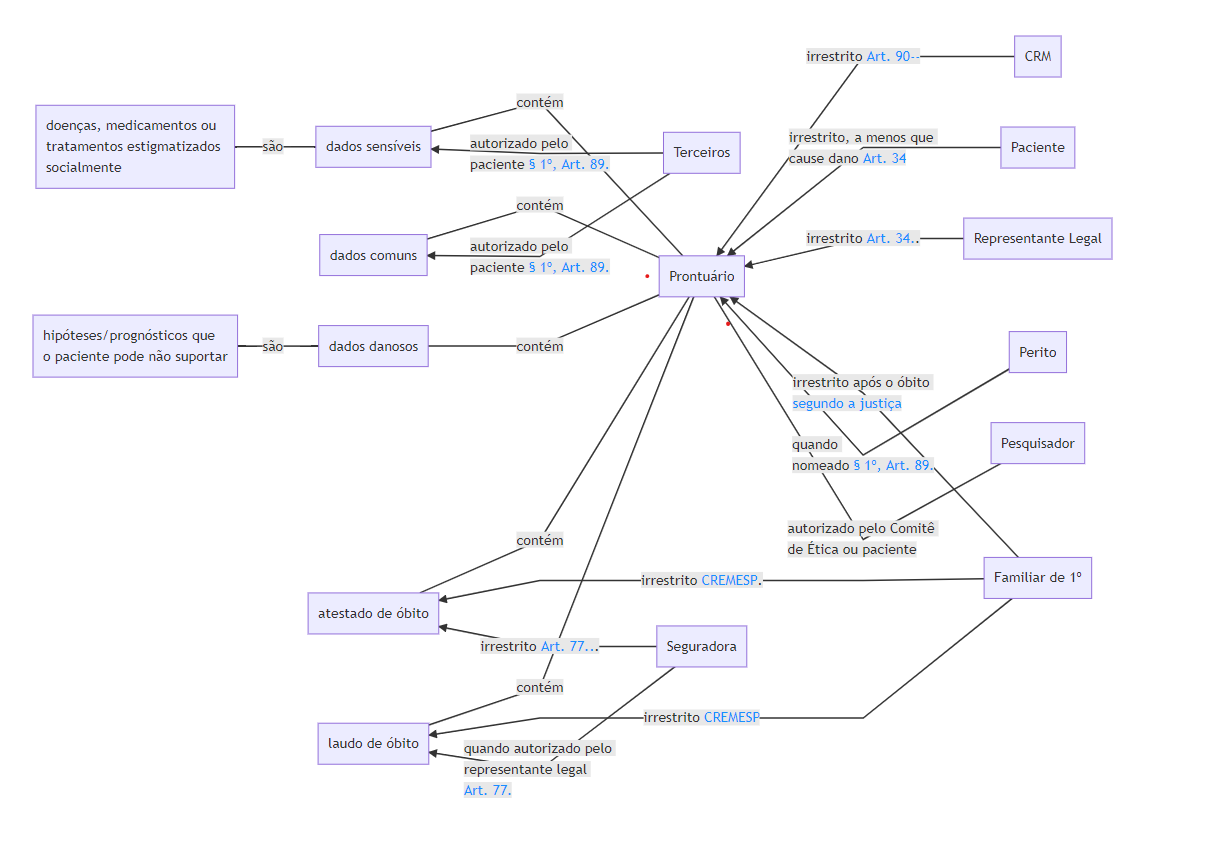
\includegraphics[width=\textwidth]{images/taxonomia-de-permissoes.png}

\href{https://mermaidjs.github.io/mermaid-live-editor/#/view/eyJjb2RlIjoiZ3JhcGggUkxcbkExW0NSTV0gLS0gaXJyZXN0cml0byA8YSBocmVmPVwiXCJodHRwOi8vYml0Lmx5L0PDs2RpZ2_DiXRpY2FNZWRpY2luYSNhcnQ5MFwiXCI-QXJ0LiA5MC0tPC9hPiAtLT4gIEJbUHJvbnR1w6FyaW9dXG5CIC0tLXxjb250w6ltfCBDW2RhZG9zIHNlbnPDrXZlaXNdXG5DIC0tLXxzw6NvfCBDMVtkb2Vuw6dhcywgbWVkaWNhbWVudG9zIG91IDxicj4gdHJhdGFtZW50b3MgZXN0aWdtYXRpemFkb3MgPGJyPiBzb2NpYWxtZW50ZV1cbkIgLS0tfGNvbnTDqW18IERbZGFkb3MgY29tdW5zXVxuQiAtLS18Y29udMOpbXwgRVtkYWRvcyBkYW5vc29zXVxuRSAtLS18c8Ojb3wgRTFbaGlww7N0ZXNlcy9wcm9nbsOzc3RpY29zIHF1ZSA8YnI-IG8gcGFjaWVudGUgcG9kZSBuw6NvIHN1cG9ydGFyXVxuQiAtLS18Y29udMOpbXwgRlthdGVzdGFkbyBkZSDDs2JpdG9dXG5CIC0tLXxjb250w6ltfCBHW2xhdWRvIGRlIMOzYml0b11cbkEyW1BhY2llbnRlXSAtLSBpcnJlc3RyaXRvLCBhIG1lbm9zIHF1ZSA8YnI-IGNhdXNlIGRhbm8gPGEgaHJlZj1cIlwiaHR0cDovL2JpdC5seS9Dw7NkaWdvw4l0aWNhTWVkaWNpbmEjYXJ0MzRcIlwiPkFydC4gMzQ8L2E-IC0tPiAgQltQcm9udHXDoXJpb11cbkEzW1JlcHJlc2VudGFudGUgTGVnYWxdIC0tIGlycmVzdHJpdG8gPGEgaHJlZj1cIlwiaHR0cDovL2JpdC5seS9Dw7NkaWdvw4l0aWNhTWVkaWNpbmEjYXJ0MzRcIlwiPkFydC4gMzQuPC9hPi4gLS0-ICBCW1Byb250dcOhcmlvXVxuQTRbRmFtaWxpYXIgZGUgMcK6XSAtLSBpcnJlc3RyaXRvIDxhIGhyZWY9XCJcImh0dHA6Ly9iaXQubHkvMlQ4NWhWTVwiXCI-Q1JFTUVTUDwvYT4uIC0tPiAgRlxuQTQgLS0gaXJyZXN0cml0byBhcMOzcyBvIMOzYml0byA8YnI-PGEgaHJlZj1cIlwiaHR0cHM6Ly9nbG8uYm8vMlQyTDRSaVwiXCI-c2VndW5kbyBhIGp1c3Rpw6dhPC9hPiAtLT4gIEJcbkE0IC0tIGlycmVzdHJpdG8gPGEgaHJlZj1cIlwiaHR0cDovL2JpdC5seS8yVDg1aFZNXCJcIj5DUkVNRVNQPC9hPiAtLT4gIEdcbkE1W1NlZ3VyYWRvcmFdIC0tIGlycmVzdHJpdG8gPGEgaHJlZj1cIlwiaHR0cDovL2JpdC5seS9Dw7NkaWdvw4l0aWNhTWVkaWNpbmEjYXJ0NzdcIlwiPkFydC4gNzcuLjwvYT4uIC0tPiAgRlxuQTUgLS0gIHF1YW5kbyBhdXRvcml6YWRvIHBlbG8gPGJyPiByZXByZXNlbnRhbnRlIGxlZ2FsIDxicj48YSBocmVmPVwiXCJodHRwOi8vYml0Lmx5L0PDs2RpZ2_DiXRpY2FNZWRpY2luYSNhcnQ3N1wiXCI-QXJ0LiA3Ny48L2E-IC0tPiAgR1xuQTZbUGVyaXRvXSAtLSBxdWFuZG8gPGJyPiBub21lYWRvIDxhIGhyZWY9XCJcImh0dHA6Ly9iaXQubHkvQ8OzZGlnb8OJdGljYU1lZGljaW5hI2FydDg5cDFcIlwiPiAmIzE2NyAxwrosIEFydC4gODkuPC9hPiAtLT4gQlxuQTdbUGVzcXVpc2Fkb3JdIC0tIGF1dG9yaXphZG8gcGVsbyBDb21pdMOqIDxicj4gZGUgw4l0aWNhIG91IHBhY2llbnRlIC0tLSBCXG5BOFtUZXJjZWlyb3NdIC0tIGF1dG9yaXphZG8gcGVsbyA8YnI-IHBhY2llbnRlIDxhIGhyZWY9XCJcImh0dHA6Ly9iaXQubHkvQ8OzZGlnb8OJdGljYU1lZGljaW5hI2FydDg5XCJcIj4gJiMxNjcgMcK6LCBBcnQuIDg5LjwvYT4gLS0-IENcbkE4W1RlcmNlaXJvc10gLS0gYXV0b3JpemFkbyBwZWxvIDxicj4gcGFjaWVudGUgPGEgaHJlZj1cIlwiaHR0cDovL2JpdC5seS9Dw7NkaWdvw4l0aWNhTWVkaWNpbmEjYXJ0ODlcIlwiPiAmIzE2NyAxwrosIEFydC4gODkuPC9hPiAtLT4gRCIsIm1lcm1haWQiOnsidGhlbWUiOiJkZWZhdWx0Iiwic2VjdXJpdHlMZXZlbCI6Imxvb3NlIn19}{Link do Diagrama (Ainda vou desenhar isso usando a biblioteca TikZ}

(quando eu refizer esse diagrama, vou incluir o MÉDICO. Esqueci do papel principal, mas já sei que ele tem acesso irrestrito se ele for o responsável pelo paciente)}

{\color{ForestGreen}Explicar que no sistema proposto existe um servidor de atributos ao qual se pedem as chaves públicas/privadas para realizar a encriptação/decriptação (1 parágrafo).} 

Atributos são pares de chaves pública e um conjunto de chaves privadas pessoais que possibilitam a criptografia assimétrica. Um atributo precisa ser publicado na blockchain para ser utilizado pelos outros usuários, e considera-se publicado o atributo que tenha seus parâmetros de chave pública enviados ao Smart Contract que gerencia estas chaves. De posse da chave pública é possível criptografar um arquivo com uma política de acesso descrita em termos daqueles atributos e caso o usuário possua as respectivas chaves privadas pessoais também é possível descriptografar o conteúdo cifrado. As operações criptográficas sempre ocorrem localmente para evitar a exposição de informação sensível à rede a qual está conectado.

{\color{ForestGreen}Explicar como é realizado o passo-a-passo para o pedido/entrega das chaves (note que aqui a descrição é muito mais profunda que o que foi mencionado na visão geral) (1 parágrafo).} 

O conjunto de chaves privadas pessoais deriva de uma chave privada secreta associada a um atributo público e de posse do certificador que a gerou. Para assegurar a unicidade da chave, também é necessário derivar a chave a partir de um identificador único (ID) associado ao usuário. Utilizar atributos com ID distintos impede a descriptografia de funcionar, assegurando que atributos não sejam intercambiáveis entre os usuários. {\color{RoyalBlue} existe um nome para esse problema onde alguém tentar ceder credenciais para alguém não autorizado. Usar aquela definição aqui} 

O mecanismo de derivação de chaves privadas pessoais está atrelado ao processamento de requisições, impedindo o certificador de conceder chaves arbitrariamente, mas somente a partir de requisição prévia. Isso é uma estratégia para limitar o poder do certificador em criar atributos, e dessa forma abusar de sua autoridade para conceder acesso indevido a agentes não autorizados de forma. O certificador portanto consulta a blockchain para obter novas requisições e decide se irá processá-la ou não. Nos dois casos, a resposta retorna à blockchain assim que a chave é criada ou quando sua criação é negada, quer seja por decisão do certificação ou por falha devido a parâmetros incorretos. 


\subsection{Contratos inteligentes com CBA}

Foram desenvolvidos cinco contratos inteligentes que permitem a autenticação, entrega de permissões e armazenamento de metadados dos prontuários eletrônicos dos pacientes. A seguir serão explicados cada um deles.


{\color{ForestGreen} Explicação do  SmartDCPABEAuthority (3 parágrafos). Ver abaixo os 3 parágrafos destrinchados.}

{\color{Magenta} 1 parágrafo para explicar o que faz o contrato (el linhas gerais).}

{\color{Magenta} Inserir o código da linha 7 até 20.}

{\color{Magenta} 1 parágrafo para explicar para que serve CADA UM dos structs, events e atributos. Exemplo. O struct X permite armazenar dados que servirão para Y. O atributo V armazena informações de W que servirão para Z.}


{\color{ForestGreen} Explicação do  SmartDCPABEKeys (3 parágrafos). Ver abaixo os 3 parágrafos destrinchados.}

{\color{Magenta} 1 parágrafo para explicar o que faz o contrato (el linhas gerais).}

{\color{Magenta} Inserir o código da linha 6 até 24.}

{\color{Magenta} 1 parágrafo para explicar para que serve CADA UM dos structs, events e atributos.}

{\color{ForestGreen} Explicação do  SmartDCPABEFiles  (3 parágrafos). Ver abaixo os 3 parágrafos destrinchados.}

{\color{Magenta} 1 parágrafo para explicar o que faz o contrato (el linhas gerais).}

{\color{Magenta} Inserir o código da linha 6 até 39.}

{\color{Magenta} 1 parágrafo para explicar para que serve CADA UM dos structs, events e atributos.}


{\color{ForestGreen} Explicação do  SmartDCPABERequests  (3 parágrafos). Ver abaixo os 3 parágrafos destrinchados.}

{\color{Magenta} 1 parágrafo para explicar o que faz o contrato (el linhas gerais).}

{\color{Magenta} Inserir o código da linha 6 até 35.}

{\color{Magenta} 1 parágrafo para explicar para que serve CADA UM dos structs, events e atributos.}


{\color{ForestGreen} Explicação do  SmartDCPABEUsers  (3 parágrafos). Ver abaixo os 3 parágrafos destrinchados.}

{\color{Magenta} 1 parágrafo para explicar o que faz o contrato (el linhas gerais).}

{\color{Magenta} Inserir o código da linha 6 até 16.}

{\color{Magenta} 1 parágrafo para explicar para que serve CADA UM dos structs, events e atributos.}



\subsection{Arquitetura Blockchain}

Como mencionado na Seção \ref{visaogeral}, o sistema é composto por 3 componentes: cliente, servidor, e a Blockchain. A Figura X mostra o relacionamento entre esses componentes. 

{\color{ForestGreen} Fazer uma figura simples que mostre os 3 componentes interligados. }


{\color{ForestGreen} Explicar implementação do cliente (5 parágrafos). Ver abaixo os 5 parágrafos destrinchados. }

{\color{Magenta} 1 parágrafo para explicar que para realizar a conexão com a Blockchain usou o web3j (explique em 2-3 linhas o web3j).}

{\color{Magenta} 1 parágrafo para explicar as 3 linhas mais importantes do código fonte de como realizar a conexão. Explicar cada linha do código. }

{\color{Magenta} 1 parágrafo para explicar que para encriptar um documento utilizando atributos usou a dcabe.}

{\color{Magenta} 1 parágrafo para explicar as 3 linhas mais importantes do código fonte de como realizar a encriptação. Explicar cada linha do código.}

{\color{Magenta} 1 parágrafo para explicar as 3 linhas mais importantes do código fonte de como acessar um contrato inteligente. Explicar cada linha do código.}

{\color{ForestGreen} Explicar implementação do servidor (3 parágrafos). Ver abaixo os 3 parágrafos destrinchados. }

{\color{Magenta} 1 parágrafo para explicar que o servidor utiliza REST para prover os serviços via web  (explique em 2-3 o que é REST).}

{\color{Magenta} 1 parágrafo para explicar que o servidor possui o serviço para inserir um documento e para recuperar um documento.}

{\color{Magenta} 1 parágrafo para explicar que o servidor insere e recupera os prontuários eletrônicos de pacientes diretamente do seu sistema de arquivos advindos das requisições web.}


{\color{ForestGreen} Explicar implementação da Blockchain (4 parágrafos). Ver abaixo os 4 parágrafos destrinchados. }

{\color{Magenta} 1 parágrafo para explicar que a Blockchain utilizada foi a testnet (explicar que existe a main e a testnet, onde a testnet é utilizada por desenvolvedores serve para realizar implantações de teste sem dispender recursos financeiros.}

{\color{Magenta} 1 parágrafo para explicar que a rede Blockchain foi implantada em um computador usando o Ganache. Explicar o que é o ganhache e o que entrega a implantação (X mineradores? X fullnodes, etc).}

{\color{Magenta} 1 parágrafo para explicar que a Blockchain possui 5 contratos inteligentes mencionados na Seção anterior.}

{\color{Magenta} 1 parágrafo para explicar que a implantação dos contratos inteligentes usou o metamask. Explicar o que é o metamask e o que especificamente você usou dele: ver identificadores das transações, conversão de .sol para .abi. Explicar o que é .abi.}

% -------------------------------------------------------------------- %
\newpage
\section{Trabalhos Relacionados}

\subsection{Sistemas de saúde com Blockchain e CBA}

\subsection{Sistemas de saúde com CBA}
\label{sub:sec:saude-cba}

\subsection{Sistemas gerais com CBA}

Caso não hajam trabalhos na seção~\ref{sub:sec:saude-cba}.

% -------------------------------------------------------------------- %
\newpage
\section{Resultados Experimentais}



% -------------------------------------------------------------------- %
\newpage
\section{Conclusões e Trabalhos futuros}

gasto financeiro
problema energético
sugestão: hyperledger.

\bibliography{doc}
\bibliographystyle{plainnat}

% -------------------------------------------------------------------- %
\newpage
\section{Anexo I}

PESSOAL DE SAÚDE - NÍVEL SUPERIOR
\begin{enumerate}
    \item ANESTESISTA
    \item ASSISTENTE SOCIAL
    \item BIOQUÍMICO/FARMACÊUTICO
    \item CIRURGIÃO GERAL
    \item CLÍNICO GERAL
    \item ENFERMEIRO
    \item FISIOTERAPEUTA
    \item FONOAUDIÓLOGO
    \item GINECO OBSTETRA
    \item MÉDICO DE FAMÍLIA
    \item NUTRICIONISTA
    \item ODONTÓLOGO
    \item PEDIATRA
    \item PSICÓLOGO
    \item PSIQUIATRA
    \item RADIOLOGISTA
    \item SANITARISTA
    \item OUTRAS ESPECIALIDADES MÉDICAS
    \item OUTRAS OCUPAÇÕES DE NÍVEL SUPERIOR RELACIONADOS À SAÚDE
\end{enumerate}
PESSOAL DE SAÚDE - NÍVEL TÉCNICO TÉCNICO/AUXILIAR
\begin{enumerate}
    \item AUXILIAR DE ENFERMAGEM
    \item FISCAL SANITÁRIO
    \item TÉCNICO DE ENFERMAGEM
    \item TÉCNICO E AUXILIAR DE FARMÁCIA
    \item TÉCNICO E AUXILIAR DE LABORATÓRIO
    \item TÉCNICO E AUXILIAR EM NUTRIÇÃO E DIETÉTICA
    \item TÉCNICO E AUXILIAR EM FISIOTERAPIA E REABILITAÇÃO
    \item TÉCNICO E AUXILIAR EM SAÚDE ORAL
    \item TÉCNICO E AUXILIAR EM VIG SANITÁRIA E AMBIENTAL
    \item TÉCNICO E AUXILIAR EM EQUIP MÉDICO-HOSPITALARES
    \item TÉCNICO E AUXILIAR EM RADIOLOGIA MÉDICA
    \item TÉCNICO E AUXILIAR EM HEMATOLOGIA/HEMOTERAPIA
    \item TÉCNICO E AUXILIAR EM HISTOLOGIA
    \item OUTRAS OCUPAÇÕES NÍVEL TÉCNICO E AUXILIAR EM SAÚDE
\end{enumerate}
PESSOAL DE SAÚDE - QUALIFICAÇÃO ELEMENTAR
\begin{enumerate}
    \item AGENTE COMUNITÁRIO DE SAÚDE
    \item AGENTE DE SAÚDE PÚBLICA
    \item ATENDENTE DE ENFERMAGEM/AUX OPER SERV DIV E ASSEM
    \item PARTEIRA
    \item OUTRAS OCUPAÇÕES NÍVEL ELEMENTAR EM SAÚDE
\end{enumerate}
PESSOAL ADMINISTRATIVO
\begin{enumerate}
    \item ADMINISTRAÇÃO
    \item SERVIÇO DE LIMPEZA/CONSERVAÇÃO
    \item SEGURANÇA
    \item OUTRAS OCUPAÇÕES ADMINISTRATIVAS
\end{enumerate}

\end{document}
